\documentclass[tikz,border=15pt]{standalone}
\usetikzlibrary{shapes,calc,arrows,through,intersections}
\begin{document}

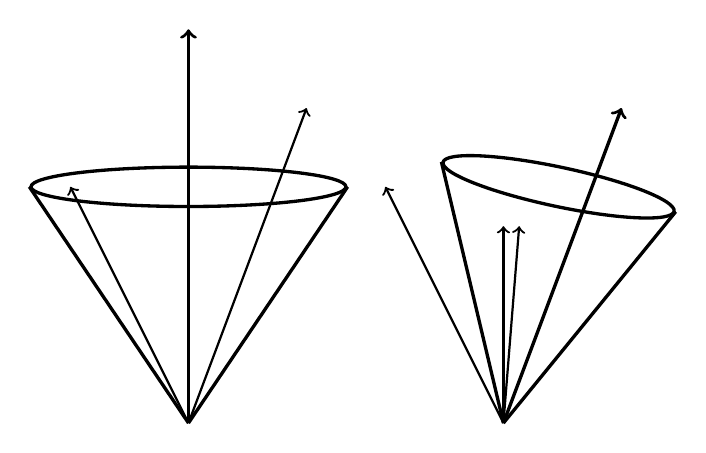
\begin{tikzpicture}

  \draw (0,3) node (jet1) [very thick,rotate=0,ellipse, minimum height=0.5cm,minimum width=4cm,draw] {};
  \draw[->, thick, ] (0,0) -- (-1.5,3);
  \draw[->, very thick, ] (0,0) -- (0,5);
  \draw[->, thick, ] (0,0) -- (1.5,4);

  \draw[very thick, ] (0,0) -- (jet1.west);
  \draw[very thick, ] (0,0) -- (jet1.east);

  \begin{scope}[shift={(4,0)}]

  \draw (0.7,3) node (jet1) [very thick,rotate=-12,ellipse, minimum height=0.5cm,minimum width=3.0cm,draw] {};
  \draw[->, thick, ] (0,0) -- (-1.5,3);
  \draw[->, thick, ] (0,0) -- (0,2.5);
  \draw[->, thick, ] (0,0) -- (0.2,2.5);
  \draw[->, very thick, ] (0,0) -- (1.5,4);

  \draw[very thick, ] (0,0) -- (jet1.west);
  \draw[very thick, ] (0,0) -- (jet1.east);


  \end{scope}

\end{tikzpicture}
\end{document}
